\documentclass{article}
\usepackage[utf8]{inputenc}
\usepackage{graphicx}
\graphicspath{ {./images/} }
\title{Voltage Divider}
\author{Zijian Xie}
\date{26 March 2020}

\begin{document}

\maketitle

\section{Circuit Schematic}
Voltage Source $Vc = 6V, R_1 = 3\Omega, R_2 = 3\Omega$.
\begin{equation}
$V_{R1} = \frac{Vc R_1}
               {R_1+R_2} = 6V x 3\Omega/(3\Omega+3\Omega) = 3V$
\end{equation}
\includegraphics[width=\textwidth, angle=-90]{01.ps}
\section{Electric Potential at point 1}
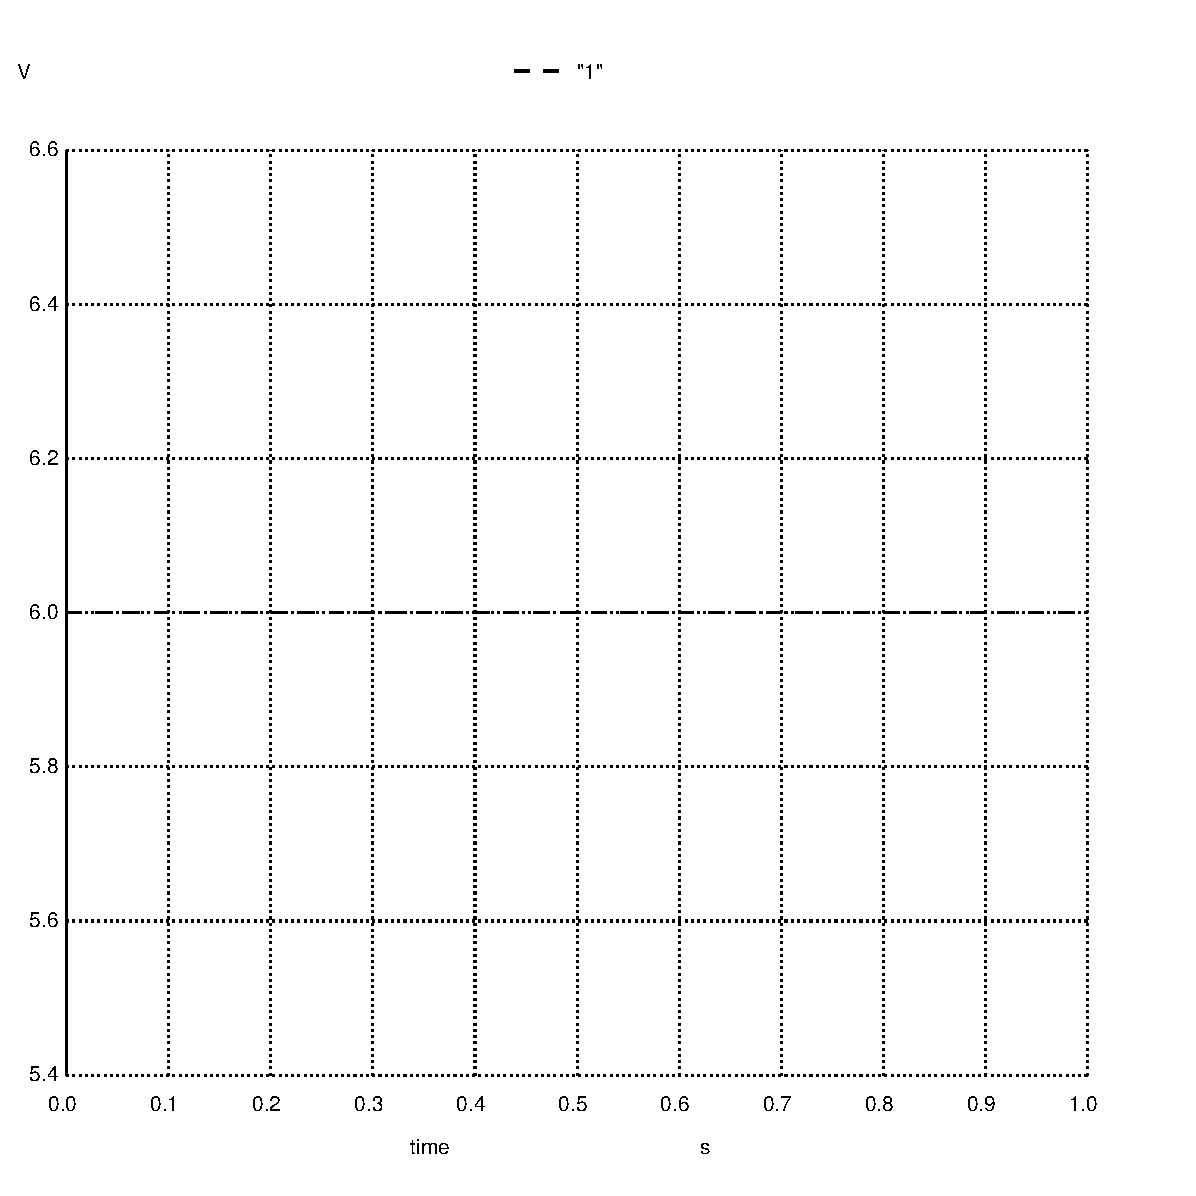
\includegraphics[width=\textwidth]{011.ps}
\section{Electric Potential at point 2}
\includegraphics[width=\textwidth]{012.ps}
\end{document}
